%%%%%%%%%%%%%%%%%%%%%%%%%%%%%%%%%%%%%%%%%%%%%%%%%%%%%%%%%%%%%%%%%%%%%%%%
\chapter{Introduction}
\label{chapter:introduction}
%%%%%%%%%%%%%%%%%%%%%%%%%%%%%%%%%%%%%%%%%%%%%%%%%%%%%%%%%%%%%%%%%%%%%%%%
\localtableofcontents

\section{Context}

Neural networks are now present all around us and in all areas.
Without knowing it, an average person uses them every day; automatic translators, chatbots, voice assistants, recommendations, etc.
The applications are very diverse and can have a profound impact on entire sectors (transport, health care, etc.).
If the use of neural networks is so important, it is because they are so effective in \emph{learning} any type of task with results that are close to perfection, surpassing man on many points.

However, although widely in use, Neural Networks are not perfect, a lot of open questions remain and many problems have emerged.
This thesis attempts to highlight and answer some of the problems that Neural Networks face.

\section{Introduction to Neural Networks}

Neural Networks find their roots, in 1958, in the works of Frank Rosenblatt \cite{rosenblatt1958perceptron} where for the first time, the Perceptron, an electronic device inspired by the human brain, showed ability to \emph{learn} from multiple examples.
In essence, the Perceptron is an algorithm for learning a binary classifier, it can be analytically described as a composition of a linear function with a threshold function as follows:
\begin{equation}
  f(\xvec) = \left\{ 
    \begin{aligned}
      &1 \quad \text{if} \quad \phi(\xvec) > 0  \\
      &0 \quad \text{otherwise}
    \end{aligned}
    \right.
\end{equation}
where $\phi(\xvec) = \theta^\top \xvec$ is a linear function.

\begin{figure}[htb]
  \centering
  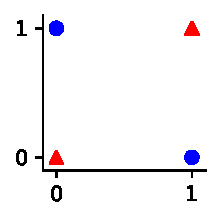
\includegraphics{figures/chapter1/xor_function.pdf}
  \caption{Graphical representation of the XOR function. This function cannot be separated by a linear classifier.}
  \label{figure:xor_function}
\end{figure}

However, a few years later after its introduction, \citet{minsky1969perceptrons} demonstrated important limitations of the Perceptron.
Indeed, although theoretical capable of classifying any linear separable problem, it is not able to correctly classify simple non-linear function (see Figure~\ref{figure:xor_function}).

One of the first Multi-Layer Perceptron or now more commonly known as \emph{Deep Neural Network} was introduced by~\citeauthor{ivakhnenko1967cybernetics} in~\citeyear{ivakhnenko1967cybernetics}.
More precisely, a Neural Neural can be analytically described as a composition of linear function interleaved with non-linear function (also called activation function):
\begin{equation}
  f_\theta(\xvec) = \phi_{\theta_L} \circ \rho \circ \phi_{\theta_{L-1}} \circ \cdots \circ \phi_{\theta_2} \circ \rho \circ \phi_{\theta_1}(\xvec)
  \label{equation:neural_network}
\end{equation}
where the function $\phi_{\theta_i}$ is a linear function parameterized by $\theta_i$, $\rho$ is an non-linear function (also called activation function), $\theta = \{\theta_1, \dots, \theta_L \}$ and $L$ correspond to the \emph{depth} of the network (\ie the number of layers).

In recent years, Deep Neural Networks have achieve state of the art performances in a variety of domains such as image recognition~\cite{lecun1998gradient,krizhevsky2012imagenet,He_2016_CVPR,tan2019efficientnet}, image detection~\cite{redmon2016you}, natural language processing~\cite{radford2018Language}, speech recognition~\cite{hinton2012deep}, etc. 
In order for Deep Neural Networks to achieve such impressive performance, specific architectures has been devised for each applications.
More precisely, each of these architectures relies on specific \emph{structured linear transformations}.


\section{Introducing Structure into Deep Neural Networks}

xxx







\section{Main contributions the Thesis}

First, in Chapter~\ref{chapter:diagonal_circulant_neural_network}, we study deep diagonal circulant neural networks, which are deep neural networks in which weight matrices are the product of diagonal and circulant ones.
Besides making a theoretical analysis of their expressivity, we introduce principled techniques for training these models: we devise an initialization scheme and propose a smart use of non-linearity functions in order to train deep diagonal circulant networks. 
Furthermore, we show that these networks outperform recently introduced deep networks with other types of structured layers. We conduct a thorough experimental study to compare the performance of deep diagonal circulant networks with state-of-the-art models based on structured matrices and with dense models. We show that our models achieve better accuracy than other structured approaches while requiring 2x fewer weights than the next best approach. Finally, we train compact and accurate deep diagonal circulant networks on a real world video classification dataset with over 3.8 million training examples. 


Finally, in Chapter~\ref{chapter:lipschitz_bound}, we tackle the problem of Lipschitz regularization of Convolutional Neural Networks.
Lipschitz regularity is now established as a key property of modern deep learning with implications in training stability, generalization, robustness against adversarial examples, etc.
However, computing the exact value of the Lipschitz constant of a neural network is known to be NP-hard.
Recent attempts from the literature introduce upper bounds to approximate this constant that are either efficient but loose or accurate but computationally expensive.
In this work, by leveraging the theory of Toeplitz matrices, we introduce a new upper bound for convolutional layers that is both tight and easy to compute.
Based on this result we devise an algorithm to train Lipschitz regularized Convolutional Neural Networks.


